% aqui comeca o texto propriamente dito

% introducao
\chapter{Introduction}

The main characteristic of massively multiplayer online games is the large number of players, having dozens, or even hundreds, of thousands of participants simultaneously. This large number of players interacting with one another generates a traffic on the support network which may grow quadratically compared to the number of players \cite{chen2006gta}, in the worst case (Figure \ref{fig:quadratic}).

\begin{figure}
  \centering
  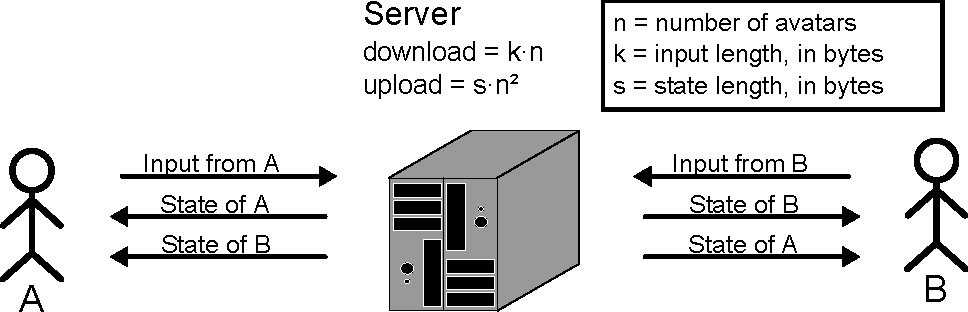
\includegraphics[width=0.6\linewidth]{images/quadratic}
  \caption{Quadratic growth of traffic when avatars are close to each other}
  \label{fig:quadratic}
\end{figure}

When using a client-server architecture, it is necessary that the server intermediates the communication between each pair of players -- assuming that the game is intended to provide guarantees of consistency and resistance to cheating. Obviously, this server will have a large communication load, thus, it must have enough resources (available bandwidth) to meet the demand of the game. For this reason, it must be considered that the main resource to analyse is the available bandwidth, for this is the current bottleneck for MMOGs \cite{feng2007wnn}.

The problem is that, when using a distributed server, it must be delegated to each server node a load proportional to its power. Thus, no matter to which server each player is connected, their game experience will be similar, regarding the response time for their actions and the time it takes to be notified of actions from other players as well as of state changes in the virtual environment of the game.
	
An initial idea might be to distribute the players among servers, so that the number of players on each server would be proportional to that server's bandwidth. However, this distribution would not work, for the burden caused by players also depends on how they are interacting with one another. For example, if the avatars of two players are too distant from each other, probably there will be no interaction between them and therefore the server needs only to update each one of them with the result of their own actions. However, if these avatars are close to each other, each player should be updated not only about the results of his own actions, but also of the actions of the other player.
	
Normally, players can freely move their avatars throughout the game world. This makes possible the formation of \emph{hotspots} \cite{ahmed2008mol}, around which the players are more concentrated than in other regions of the virtual environment (Figure \ref{fig:avatarsdistribution}). Moreover, many massively multiplayer online RPGs not only permit but also stimulate, to some extent, the formation of these points of interest. In the worlds of these MMORPGs, there are entire cities, where the players meet to chat, exchange virtual goods or even fight, and there are also desertic areas, with few attractions for the players, and where the number of avatars is relatively small compared to other places of the environment.

\begin{figure}
  \centering
  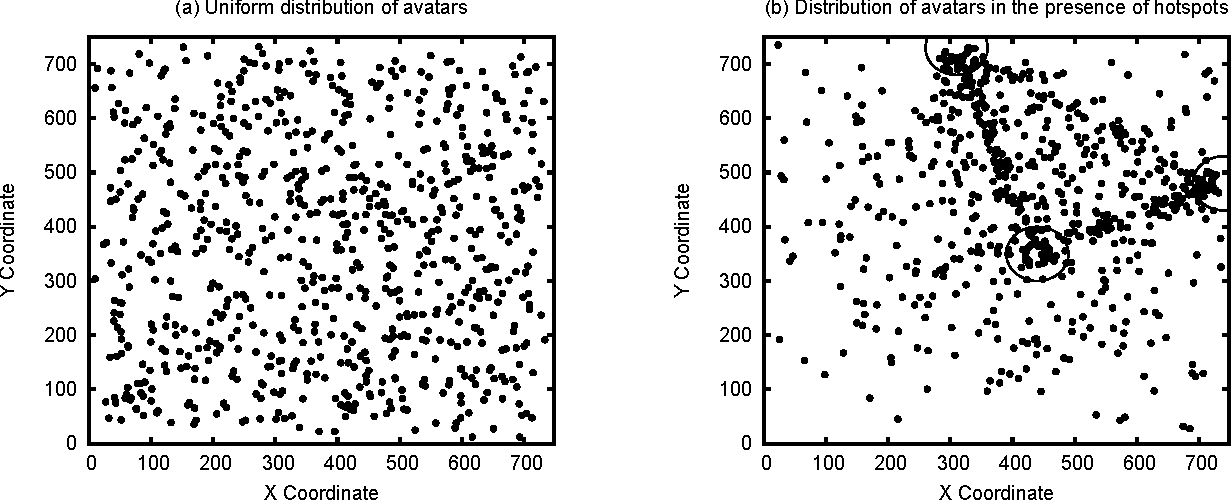
\includegraphics[width=1.0\linewidth]{images/avatarsdistribution}
  \caption{Distribution of avatars with and without hotspots}
  \label{fig:avatarsdistribution}
\end{figure}

For this reason, it is not enough just to divide the players between servers, even if this division is proportional to the resources of each one of them. First, in some cases the usage of the server's bandwidth may be square to the number of players, while in others it may be linear. It is shown in \cite{chen2006gta} that, in a group of avatars who are neighbors of one another, the rate of packets sent to each player is proportional to the number of avatars in that group (as in Fig. \ref{fig:quadratic}). This reason alone is enough to define a new criterion for load balancing.

Moreover, there is another important issue: the overhead of the distribution. As the servers need to communicate with one another, there must be a way to minimize this traffic, reducing the waste of resources of the server system. The load balancing scheme for MMOGs must, then, prevent the presence of hotspots from degrading the quality of the game beyond a tolerable limit.

In this work, it is presented a few recent papers which try to solve this problem, achieving a significant fair load distribution. Besides reviewing these works, some comments are added based on the advantages and weaknesses of each solution presented by the authors. In the end of this paper, a new idea is presented, suggesting the use of a generic binary space partition (BSP) tree.